\newcommand{\componentA}{0.9451}
\newcommand{\componentB}{0.9804}
\newcommand{\componentC}{0.9961}

\definecolor{macros}{rgb}{\componentA, \componentB, \componentC}
\definecolor{tikz}{rgb}{  \componentB, \componentC, \componentA}
\definecolor{auto}{rgb}{  \componentB, \componentA, \componentC}
\definecolor{next}{rgb}{  \componentA, \componentC, \componentB}
\definecolor{errors}{rgb}{    \componentC, \componentA, \componentB}
\definecolor{templates}{rgb}{ \componentC, \componentB, \componentA}
\definecolor{exercises}{rgb}{ \componentA, \componentB, \componentC}

\newcommand{\bgcolor}{Purple} % this should be renewed below

%%%%%%%%%%%%%%%%%%%%%%%%%%%%%%%%%%%%%%%%%%%%%%%%%%%%%%%%%%%%%%%
%%%%%%%%%%%%%%%%%%%%%%%%%%%%%%%%%%%%%%%%%%%%%%%%%%%%%%%% Macros

% background color pre
{
\setbeamercolor{background canvas}{bg=macros}
\renewcommand{\bgcolor}{macros}

\section{Macros}
\begin{frame}
  \vspace{25mm}
  \begin{center}
    \Huge{Part 1:\\Macros}
  \end{center}
\end{frame}

\subsection{Introduction}
\begin{frame}[fragile]
  \frametitle{Introduction}
  \vspace{3mm}
  \textbf{Q:} What is a macro?
  
  \pause
  \vspace{5mm}
  \textbf{A:} It is a bit like a function, but the evaluation of the body is done by replacing all occurrences of the parameters with the concrete arguments. The resulting text is inserted in the macro calls place.
  
  \pause
  \vspace{5mm}
  \textbf{Consequence:} It can be tricky to think about nested macros, and worse to reason about errors in them.
  
  \pause
  \vspace{5mm}
  As the old adage goes, if your macro definitions represents your peak brilliance, then you are mentally incapable of debugging them.
\end{frame}

\subsection{Keyword Markup}
\begin{frame}[fragile]
  \frametitle{Keyword Markup}
  \vspace{3mm}
  \textbf{Pattern:} I want to place certain words in the index, and make it clear that they are special.
  
  \vspace{5mm}
  \textbf{Definition:}
  \begin{minted}[breaklines]{latex}
\newcommand{\idx}[2]{\index{#2}\textcolor{purple}{#1}}
  \end{minted}
  
  \vspace{5mm}
  \textbf{Use:}
  \begin{minted}[breaklines]{latex}
We need to fit this to the \idx{tradeoff}{Tradeoff}.
  \end{minted}
  
  \vspace{5mm}
  \textbf{Appearance:} \\
  We need to fit this to the \idx{tradeoff}{Tradeoff}.
\end{frame}

\subsection{Highlights}
\begin{frame}[fragile]
  \frametitle{Highlights}
  \vspace{3mm}
  \textbf{Pattern:} I need to refer to something of a particular type (e.g., a file, variable or type), and want it to stand out.
  
  \vspace{5mm}
  \textbf{Definition:}
  \begin{minted}[breaklines]{latex}
\newcommand{\filename}[1]{ \textcolor{purple}{\texttt{#1}} }
  \end{minted}
  
  \vspace{5mm}
  \textbf{Use:}
  \begin{minted}[breaklines]{latex}
The configuration is pulled from the \filename{conf.yaml} file.
  \end{minted}
  
  \vspace{5mm}
  \textbf{Appearance:}
  \\
  The configuration is pulled from the \textcolor{purple}{\texttt{conf.yaml}} file.
\end{frame}

\subsection{Description Lists}
\begin{frame}[fragile]
  \frametitle{Description Lists}
  \vspace{0mm}
  \textbf{Pattern:} List items often need a header that is emphasized over the rest of the item text.
  
  \vspace{3mm}
  \textbf{Definition:}
  \begin{minted}[breaklines]{latex}
\newcommand{\textdesc}[1]{ \textit{\textbf{#1}} }
\newcommand{\descitem}[1]{ \item \textdesc{#1} }
  \end{minted}
  
  \vspace{2mm}
  \textbf{Use:}
  \begin{minted}[breaklines]{latex}
\begin{itemize}
  \descitem{Bonobo} An intelligent ape.
  \descitem{Gibbon} An agile ape.
\end{itemize}
  \end{minted}
  
  \vspace{2mm}
  \textbf{Appearance:}
  \begin{itemize}
    \descitem{Bonobo} An intelligent ape.
    \descitem{Gibbon} An agile ape.
  \end{itemize}
\end{frame}

\subsection{Inspirational Quotes}
\begin{frame}[fragile]
  \frametitle{Inspirational Quotes [1/2]}
  \vspace{3mm}
  \textbf{Pattern:} I want to sprinkle inspirational quotes around my document.
  
  \vspace{5mm}
  \textbf{Definition:}
  \begin{minted}[breaklines]{latex}
\newenvironment{inspiration}[2][0.9]
{
  \begin{center}
  \newcommand{\saveme}{#2}
  \begin{minipagewithmarginpars}{#1\textwidth}
}
{
  
  \raggedleft{--- \textsl{\saveme}}
  \end{minipagewithmarginpars}
  \end{center}
}
  \end{minted}
\end{frame}
\begin{frame}[fragile]
  \frametitle{Inspirational Quotes [2/2]}
  \vspace{3mm}
  \textbf{Use:}
  \begin{minted}[breaklines]{latex}
\begin{inspiration}{Jane Goodall}
  You cannot get through a single day without having an impact on the
  world around you. What you do makes a difference, and you have to
  decide what kind of difference you want to make.
\end{inspiration}
  \end{minted}
  
  \vspace{5mm}
  \textbf{Appearance:}
  \begin{inspiration}{Jane Goodall}
  You cannot get through a single day without having an impact on the world around you. What you do makes a difference, and you have to decide what kind of difference you want to make.
  \end{inspiration}
\end{frame}

\subsection{Typed Boxes}
\begin{frame}[fragile]
  \frametitle{Typed Boxes [1/2]}
  \vspace{3mm}
  \textbf{Pattern:} I want certain text to be placed in special boxes (e.g., info or conclusion).
  
  \vspace{5mm}
  \textbf{Definition:}
  \begin{minted}[breaklines,fontsize=\footnotesize]{latex}
\newenvironment{tbox}[2][0.9]
{
  \begin{center}
    \begin{tabular}{|p{#1\textwidth}|}
      \hline
      \cellcolor[gray]{0.9}
      \textbf{#2} \\
      \hline
      \cellcolor[gray]{0.95}
}{
      \\
      \hline
    \end{tabular}
  \end{center}
}
  \end{minted}
\end{frame}
\begin{frame}[fragile]
  \frametitle{Typed Boxes [2/2]}
  \vspace{3mm}
  \textbf{Use:}
  \begin{minted}[breaklines]{latex}
\begin{tbox}{Intuition}
  The dispatch mechanism is highly concurrent. It might not
  bottleneck the system.
\end{tbox}
  \end{minted}
  
  \vspace{5mm}
  \textbf{Appearance:}
  \begin{tbox}{Intuition}
    The dispatch mechanism is highly concurrent. It might not bottleneck the system.
  \end{tbox}
\end{frame}

% background color post
}

%%%%%%%%%%%%%%%%%%%%%%%%%%%%%%%%%%%%%%%%%%%%%%%%%%%%%%%%%%%%%
%%%%%%%%%%%%%%%%%%%%%%%%%%%%%%%%%%%%%%%%%%%%%%%%%%%%%%%% tikz

% background color pre
{
\setbeamercolor{background canvas}{bg=tikz}
\renewcommand{\bgcolor}{tikz}

\section{TikZ}
\begin{frame}
  \vspace{25mm}
  \begin{center}
    \Huge{Part 2:\\\TikZ}
  \end{center}
\end{frame}

\subsection{The \envname{tikzpicture} Environment}
\begin{frame}[fragile]
  \frametitle{The \envname{tikzpicture} Environment}
  \vspace{3mm}
  Load \TikZ\ package:
  \begin{minted}[fontsize=\normalsize]{latex}
\usepackage{tikz}
  \end{minted}
  
  \pause
  \vspace{9mm}
  Then we get access to the \envname{tikzpicture} environment:
  \vspace{16mm}
  \begin{minted}[fontsize=\normalsize,escapeinside=||]{latex}
\begin{tikzpicture}[|\tikzmark{parbefore}|    |\tikzmark{parafter}|]
|\tikzmark{contents}|

\end{tikzpicture}
  \end{minted}
  \begin{tikzpicture}[remember picture]
    \tikzstyle{arrow} = [thick,->,>=stealth, draw=black]
    \tikzstyle{box} = [overlay,rectangle,thick,draw=black]
    \tikzstyle{direction}=[
      overlay,
      rectangle,
      anchor=north west,
      pattern=north east lines,
      even odd rule,
      thick,
      font=\bfseries,
      minimum width=\textwidth,
      minimum height=10.5mm,
    ]
    \tikzstyle{contents}=[direction,pattern color=purple!60,draw=purple]
    
    \coordinate (par_coord) at ([yshift= 1.1mm] $(pic cs:parbefore)!0.5!(pic cs:parafter)$);
    
    \pause
    \node[box,minimum width=11mm, minimum height=4mm] (par_box)
      at (par_coord) {};
    \node[overlay,anchor=south] (par_label)
      at ([yshift=6mm] par_box.north) {parameters};
    \draw[overlay, arrow, thick] (par_label) -- (par_box);
    
    \pause
    \node[contents] () at ([yshift=4mm] pic cs:contents) {Contents};
  \end{tikzpicture}
\end{frame}

\subsection{Coordinate System}
\begin{frame}[fragile]
  \frametitle{Coordinate System}
  \vspace{3mm}
  \begin{center}
    \begin{tikzpicture}[]
      \newcommand{\size}[0]{ 6cm }
      \tikzstyle{dedge} = [thick,->,>=stealth,draw=black]
      \draw[dedge] (0,0) -- (\size,0) node[midway,below]  {\textsl{\textcolor{purple}{x}}};
      \draw[dedge] (0,0) -- (0,\size) node[midway,left] {\textsl{\textcolor{purple}{y}}};
    \end{tikzpicture}
  \end{center}
\end{frame}

\subsection{Nodes}
\begin{frame}[fragile]
  \frametitle{Nodes}
  \vspace{3mm}
  A \textsl{node} is something that you can place at a specific position.
  
  \vspace{5mm}
  That something is typically some text, but images and math is also allowed.
  
  \pause
  \vspace{5mm}
  Properties:
  \begin{itemize}
    \item This material is placed at the \textsl{anchor point} of the node.
    \item A shape can be drawn around it: circle, rectangle, diamond \ldots
    \item The shape itself is drawn according to a \textsl{style}.
    \item The inside of that shape can be filled with a color or patters.
    \item All of this is \textsl{drawn} according to a \textsl{style}.
  \end{itemize}
\end{frame}

\subsubsection{The Page}
\begin{frame}[fragile]
  \frametitle{Nodes \subpart{The Page}}
  \vspace{3mm}
  Within the \envname{tikzpicture} environment one node is defined: \say{\texttt{current page}}.
  
  \vspace{5mm}
  This node is completely transparent and has the shape and position of the \textsl{current page}.
  
  \vspace{5mm}
  Often, it makes sense to use this node of positioning rather than relying on the current location on the page.
  \begin{itemize}
    \item This makes the positioning absolute (relative to the page) rather than relative (relative to the cursor position).
  \end{itemize}
\end{frame}

\subsubsection{Anchor Points}
\begin{frame}[fragile]
  \frametitle{Nodes \subpart{Anchor Points}}
  \vspace{3mm}
  \begin{tikzpicture}[remember picture, overlay]
    \newcommand{\pointname}[1]{ \texttt{#1} }
    \tikzstyle{dedge} = [thick,->,>=stealth,draw=black]
    
    \tikzstyle{point}=[
      circle,
      draw=purple,
      fill=purple!5,
      anchor=center,
      minimum size=1.2mm,
      inner sep=0pt,
      thick,
    ]
    
    \coordinate (squarecoord) at ([xshift=-3.8cm] current page.center);
    \coordinate (circlecoord) at ([xshift=3.8cm] current page.center);
    
    \node[rectangle,draw,minimum height=2.6cm,minimum width=2.6cm] (square) at (squarecoord) {};
    \node[circle,draw,minimum height=2.6cm,minimum width=2.6cm] (circle) at (circlecoord) {};
    
    \only<2>{
      \node[point] (sc) at (square.center) {};
      \node[point] (cc) at (circle.center) {};
      \node[anchor=north] () at (sc.south) {\pointname{center}};
      \node[anchor=north] () at (cc.south) {\pointname{center}};
      
      \node[point] (sn) at (square.north) {};
      \node[point] (cn) at (circle.north) {};
      \node[anchor=south] () at (sn.north) {\pointname{north}};
      \node[anchor=south] () at (cn.north) {\pointname{north}};
      
      \node[point] (ss) at (square.south) {};
      \node[point] (cs) at (circle.south) {};
      \node[anchor=north] () at (ss.south) {\pointname{south}};
      \node[anchor=north] () at (cs.south) {\pointname{south}};
      
      \node[point] (se) at (square.east) {};
      \node[point] (ce) at (circle.east) {};
      \node[anchor=west] () at (se.east) {\pointname{east}};
      \node[anchor=west] () at (ce.east) {\pointname{east}};
      
      \node[point] (sw) at (square.west) {};
      \node[point] (cw) at (circle.west) {};
      \node[anchor=east] () at (sw.west) {\pointname{west}};
      \node[anchor=east] () at (cw.west) {\pointname{west}};
      
      \node[point] (snw) at (square.north west) {};
      \node[point] (cnw) at (circle.north west) {};
      \node[anchor=south east] () at (snw.north west) {\pointname{north west}};
      \node[anchor=south east] () at (cnw.north west) {\pointname{north west}};
      
      \node[point] (sne) at (square.north east) {};
      \node[point] (cne) at (circle.north east) {};
      \node[anchor=south west] () at (sne.north east) {\pointname{north east}};
      \node[anchor=south west] () at (cne.north east) {\pointname{north east}};
      
      \node[point] (ssw) at (square.south west) {};
      \node[point] (csw) at (circle.south west) {};
      \node[anchor=north east] () at (ssw.south west) {\pointname{south west}};
      \node[anchor=north east] () at (csw.south west) {\pointname{south west}};
      
      \node[point] (sse) at (square.south east) {};
      \node[point] (cse) at (circle.south east) {};
      \node[anchor=north west] () at (sse.south east) {\pointname{south east}};
      \node[anchor=north west] () at (cse.south east) {\pointname{south east}};
    }
  \end{tikzpicture}
\end{frame}

\subsubsection{Positioning of Rectangles}
\begin{frame}[fragile]
  \frametitle{Nodes \subpart{Positioning of Rectangles}}
  \pause
  \begin{tikzpicture}[remember picture, overlay]
    \newcommand{\squaresize}[0]{ 32mm }
    \newcommand{\pointname}[1]{ \texttt{#1} }
    
    \tikzstyle{point}=[
      circle,
      draw=purple,
      fill=purple!5,
      anchor=center,
      minimum size=1.2mm,
      inner sep=0pt,
      thick,
    ]
    \tikzstyle{rect}=[
      rectangle,
      draw=black,
      anchor=center,
      minimum width=2*\squaresize,
      minimum height=\squaresize,
      thick,
    ]
    
    \coordinate (anchor) at (current page.center);
    
    \only<3->{
      \node[rect,anchor=south east] () at (anchor) {
        \mintinline[fontsize=\tiny]{latex}{\node[rect,anchor=south east] () at (anchor) {};}
      };
    }
    \only<4->{
      \node[rect,anchor=south west] () at (anchor) {
        \mintinline[fontsize=\tiny]{latex}{\node[rect,anchor=south west] () at (anchor) {};}
      };
    }
    \only<5->{
      \node[rect,anchor=north west] () at (anchor) {
        \mintinline[fontsize=\tiny]{latex}{\node[rect,anchor=north west] () at (anchor) {};}
      };
    }
    \only<6->{
      \node[rect,anchor=north east] () at (anchor) {
        \mintinline[fontsize=\tiny]{latex}{\node[rect,anchor=north east] () at (anchor) {};}
      };
    }
    
    \node[point] () at (anchor) {};
    
    \node[anchor=north east] () at (current page.north east) {
      \mintinline[fontsize=\tiny]{latex}{\coordinate (anchor) at (current page.center);}
    };
  \end{tikzpicture}
\end{frame}

\subsubsection{Positioning of Circles}
\begin{frame}[fragile]
  \frametitle{Nodes \subpart{Positioning of Circles}}
  \pause
  \begin{tikzpicture}[remember picture, overlay]
    \newcommand{\squaresize}[0]{ 32mm }
    \newcommand{\pointname}[1]{ \texttt{#1} }
    
    \tikzstyle{point}=[
      circle,
      draw=purple,
      fill=purple!5,
      anchor=center,
      minimum size=1.2mm,
      inner sep=0pt,
      thick,
    ]
    \tikzstyle{circ}=[
      circle,
      draw=black,
      anchor=center,
      minimum width=2*\squaresize,
      minimum height=\squaresize,
      thick,
    ]
    
    \coordinate (anchor) at (current page.center);
    
    \only<3->{
      \node[circ,anchor=south east] () at (anchor) {
        \mintinline[fontsize=\tiny]{latex}{\node[circ,anchor=south east] () at (anchor) {};}
      };
    }
    \only<4->{
      \node[circ,anchor=south west] () at (anchor) {
        \mintinline[fontsize=\tiny]{latex}{\node[circ,anchor=south west] () at (anchor) {};}
      };
    }
    \only<5->{
      \node[circ,anchor=north west] () at (anchor) {
        \mintinline[fontsize=\tiny]{latex}{\node[circ,anchor=north west] () at (anchor) {};}
      };
    }
    \only<6->{
      \node[circ,anchor=north east] () at (anchor) {
        \mintinline[fontsize=\tiny]{latex}{\node[circ,anchor=north east] () at (anchor) {};}
      };
    }
    
    \node[point] () at (anchor) {};
    
    \node[anchor=north east] () at (current page.north east) {
      \mintinline[fontsize=\tiny]{latex}{\coordinate (anchor) at (current page.center);}
    };
  \end{tikzpicture}
\end{frame}

\subsection{Coordinates}
\begin{frame}[fragile]
  \frametitle{Coordinates}
  \vspace{3mm}
  A coordinate is a convenience construct. It allows you to define a coordinate without a node.
  
  \pause
  \vspace{5mm}
  For instance, we can define an offsat center:
  \begin{minted}[fontsize=\normalsize]{latex}
\coordinate (center) at ([yshift=-12mm] current page.center);
  \end{minted}
  
  \pause
  \vspace{5mm}
  And then future positions can be based on this \texttt{center} definition instead of something more complex:
  \begin{minted}[fontsize=\normalsize]{latex}
\node[rectangle,anchor=east] () at ([xshift=-2mm] center) {left};
\node[rectangle,anchor=west] () at ([xshift= 2mm] center) {right};
  \end{minted}
  
  \pause
  \vspace{5mm}
  The shift can be in two dimensions:
  \begin{minted}[fontsize=\normalsize]{latex}
\node[rectangle] () at ([xshift=2mm,yshift=3cm] center) {translation};
  \end{minted}
\end{frame}

\subsection{Paths}
\begin{frame}[fragile]
  \frametitle{Paths}
  \vspace{3mm}
  
\end{frame}

\subsubsection{Node vs Points}
\begin{frame}[fragile]
  \frametitle{Paths \subpart{Node vs Points}}
  \vspace{3mm}
    \begin{tikzpicture}[remember picture,overlay]
    \newcommand{\height}[0]{42mm}
    \newcommand{\dist}[0]{5mm}
    
    \tikzstyle{edge} = [thick,draw=black]
    \tikzstyle{dedge} = [edge,->,>=stealth]
    
    \node[rectangle,thick,anchor=east,draw,minimum height=\height] (code) at ([xshift=-\dist]current page.center) {
      \begin{minipage}{6cm}
        \begin{minted}[fontsize=\scriptsize]{latex}
\node[point] (a) at
  ([xshift=-1.6cm,yshift= 8mm]anchor)
  {$N_a$};

\node[point] (b) at
  ([xshift= 1.6cm,yshift=-8mm]anchor)
  {$N_b$};

\draw[edge,draw=blue] (a)
                   -- (b);
\draw[edge,draw=red]  (a.south)
                   -- (b.south);
        \end{minted}
      \end{minipage}
    };
    
    \node[rectangle,thick,anchor=west,draw,minimum height=\height,minimum width=6.2cm] (output) at ([xshift=\dist]current page.center) {};
    
    \draw[dedge] (code)->(output);
    
    % rhs
    \tikzstyle{point}=[
      circle,
      draw=purple,
      fill=purple!5,
      thick,
      minimum height=0pt,
      anchor=center,
      minimum size=1.1cm,
    ]
    \coordinate (anchor) at (output.center);
    
    \node[point] (a)
      at ([xshift=-1.6cm,yshift= 8mm]anchor)
      {$N_a$};
    \node[point] (b)
      at ([xshift= 1.6cm,yshift=-8mm]anchor)
      {$N_b$};
    
    \draw[edge,draw=blue] (a) -- (b);
    \draw[edge,draw=red] (a.south) -- (b.south);
  \end{tikzpicture}
\end{frame}

\subsubsection{Angled Edges}
\begin{frame}[fragile]
  \frametitle{Paths \subpart{Angled Edges}}
  \begin{tikzpicture}[remember picture,overlay]
    \newcommand{\height}[0]{42mm}
    \newcommand{\dist}[0]{5mm}
    
    \tikzstyle{edge} = [thick,draw=black]
    \tikzstyle{dedge} = [edge,->,>=stealth]
    
    \node[rectangle,thick,anchor=east,draw,minimum height=\height] (code) at ([xshift=-\dist]current page.center) {
      \begin{minipage}{6cm}
        \begin{minted}[fontsize=\scriptsize]{latex}
\node[point] (a)
  at ([xshift=-1cm,yshift= 1cm]anchor)
  {$N_a$};

\node[point] (b)
  at ([xshift= 1cm,yshift=-1cm]anchor)
  {$N_b$};

\draw[edge,draw=red]  (a) -| (b);
\draw[edge,draw=blue] (a) |- (b);
        \end{minted}
      \end{minipage}
    };
    
    \node[rectangle,thick,anchor=west,draw,minimum height=\height,minimum width=6.2cm] (output) at ([xshift=\dist]current page.center) {};
    
    \draw[dedge] (code)->(output);
    
    % rhs
    \tikzstyle{point}=[
      circle,
      draw=purple,
      fill=purple!5,
      thick,
      minimum height=0pt,
      anchor=center,
      minimum size=1.1cm,
    ]
    \coordinate (anchor) at (output.center);
    
    \node[point] (a)
      at ([xshift=-1cm,yshift= 1cm]anchor)
      {$N_a$};
    \node[point] (b)
      at ([xshift= 1cm,yshift=-1cm]anchor)
      {$N_b$};
    
    \draw[edge,red]  (a) -| (b);
    \draw[edge,blue] (a) |- (b);
  \end{tikzpicture}
\end{frame}

\subsubsection{Curved Edges}
\begin{frame}[fragile]
  \frametitle{Paths \subpart{Curved Edges}}
  \begin{tikzpicture}[remember picture,overlay]
    \newcommand{\height}[0]{48mm}
    \newcommand{\dist}[0]{5mm}
    
    \tikzstyle{edge} = [thick,draw=black]
    \tikzstyle{dedge} = [edge,->,>=stealth]
    
    \node[rectangle,thick,anchor=east,draw,minimum height=\height] (code) at ([xshift=-\dist]current page.center) {
      \begin{minipage}{6cm}
        \begin{minted}[fontsize=\tiny]{latex}
\newcommand{\aI}[0]{180}
\newcommand{\aO}[0]{90}

\node[point] (a) at ([xshift=-1.6cm]anchor) {$N_a$};
\node[point] (b) at ([xshift= 1.6cm]anchor) {$N_b$};

\draw[edge]
  (a) to[out=\aO+20,in=\aI+10,looseness=3.0] (b);
\draw[edge]
  (a) to[out=\aO+10,in=\aI+ 5,looseness=2.5] (b);
\draw[edge]
  (a) to[out=\aO+ 0,in=\aI+ 0,looseness=2.0] (b);
\draw[edge]
  (a) to[out=\aO-10,in=\aI- 5,looseness=1.5] (b);
\draw[edge]
  (a) to[out=\aO-20,in=\aI-10,looseness=1.0] (b);
        \end{minted}
      \end{minipage}
    };
    
    \node[rectangle,thick,anchor=west,draw,minimum height=\height,minimum width=6.2cm] (output) at ([xshift=\dist]current page.center) {};
    
    \draw[dedge] (code)->(output);
    
    % rhs
    \tikzstyle{point}=[
      circle,
      draw=purple,
      fill=purple!5,
      thick,
      minimum height=0pt,
      anchor=center,
      minimum size=1.1cm,
    ]
    \coordinate (anchor) at (output.center);
    
    \newcommand{\aI}[0]{180}
    \newcommand{\aO}[0]{90}
    
    \node[point] (a)
      at ([xshift=-1.6cm]anchor)
      {$N_a$};
    \node[point] (b)
      at ([xshift= 1.6cm]anchor)
      {$N_b$};
    
    \draw[edge] (a) to[out=\aO+20,in=\aI+10,looseness=3] (b);
    \draw[edge] (a) to[out=\aO+10,in=\aI+ 5,looseness=2.5] (b);
    \draw[edge] (a) to[out=\aO+ 0,in=\aI+ 0,looseness=2] (b);
    \draw[edge] (a) to[out=\aO-10,in=\aI- 5,looseness=1.5] (b);
    \draw[edge] (a) to[out=\aO-20,in=\aI-10,looseness=1] (b);
  \end{tikzpicture}
\end{frame}

\subsection{Styles}
\begin{frame}[fragile]
  \frametitle{Styles}
  \vspace{3mm}
  Each node and path is drawn according to a sequence of style rules.
  
  \vspace{5mm}
  Later rules override earlier rules
  
  \vspace{5mm}
  We can define shorthands for sequences of rules, and these may refer to other such shorthands.
  
  \vspace{5mm}
  Format:
  \begin{minted}[fontsize=\normalsize,escapeinside=||]{latex}
\tikzstyle{|\tikzmark{namebefore}|dedge|\tikzmark{nameafter}|} = [|\tikzmark{rulesbefore}|thick,->,>=stealth,draw=black|\tikzmark{rulesafter}|]
  \end{minted}
  \begin{tikzpicture}[remember picture]
    \tikzstyle{arrow} = [thick,->,>=stealth, draw=black]
    \tikzstyle{box} = [overlay,rectangle,thick,draw=black]
    
    \coordinate (name_coord) at ([yshift= 1.1mm] $(pic cs:namebefore)!0.5!(pic cs:nameafter)$);
    \coordinate (rules_coord) at ([yshift= 1.1mm] $(pic cs:rulesbefore)!0.5!(pic cs:rulesafter)$);
    
    \pause
    \node[box,minimum width=11mm, minimum height=4mm] (name_box)
      at (name_coord) {};
    \node[overlay,anchor=north] (name_label)
      at ([yshift=-6mm] name_box.south) {name};
    \draw[overlay, arrow, thick] (name_label) -- (name_box);
    
    \pause
    \node[box,minimum width=63mm, minimum height=4mm] (rules_box)
      at (rules_coord) {};
    \node[overlay,anchor=north] (rules_label)
      at ([yshift=-6mm] rules_box.south) {Rules};
    \draw[overlay, arrow, thick] (rules_label) -- (rules_box);
  \end{tikzpicture}
\end{frame}

\subsubsection{Select Rules}
\begin{frame}[fragile]
  \frametitle{Styles \subpart{Select Rules}}
  \vspace{3mm}
  \begin{itemize}
    \item Name of a previously defined style. Following rules will override.
    \item Line thickness: \hldata{\texttt{thin}}, \hldata{\texttt{thick}}, \hldata{\texttt{very thick}}
    \item Anchor point: \hldata{\texttt{anchor=north west}}
    \item Stroke color: \hldata{\texttt{draw=purple}}
    \item Fill color: \hldata{\texttt{fill=purple}}
    \item Text color: \hldata{\texttt{text=purple}}
    \item Text alignment: \hldata{\texttt{align=left}} \\
          (needed for multiple lines)
    \item Node minimum width: \hldata{\texttt{minimum width=2.4cm}}
    \item Node minimum height: \hldata{\texttt{minimum height=12mm}}
    \item Padding between node text and shape: \hldata{\texttt{inner sep=0pt}}
  \end{itemize}
\end{frame}

%\subsubsection{Example}
%\begin{frame}[fragile]
%  \frametitle{Styles \subpart{Example}}
%  \vspace{3mm}
%  
%\end{frame}

\subsubsection{Use of Derived Styles}
\begin{frame}[fragile]
  \frametitle{Styles \subpart{Use of Derived Styles}}
  \begin{tikzpicture}[remember picture,overlay]
    \newcommand{\height}[0]{42mm}
    \newcommand{\dist}[0]{5mm}
    
    \tikzstyle{edge} = [thick,draw=black]
    \tikzstyle{dedge} = [edge,->,>=stealth]
    
    \node[rectangle,thick,anchor=east,draw,minimum height=\height] (code) at ([xshift=-\dist]current page.center) {
      \begin{minipage}{6cm}
        \begin{minted}[fontsize=\scriptsize]{latex}
\tikzstyle{edge} = [thick,draw=black]
\tikzstyle{dedge} = [edge,->,>=stealth]

\node[point] (a)
  at ([xshift=-2cm]anchor) {$N_a$};
\node[point] (b)
  at ([xshift= 0cm]anchor) {$N_b$};
\node[point] (c)
  at ([xshift= 2cm]anchor) {$N_c$};

\draw[edge]  (a)--(b);
\draw[dedge] (b)--(c);
        \end{minted}
      \end{minipage}
    };
    
    \node[rectangle,thick,anchor=west,draw,minimum height=\height,minimum width=6.2cm] (output) at ([xshift=\dist]current page.center) {};
    
    \draw[dedge] (code)->(output);
    
    % rhs
    \tikzstyle{point}=[
      circle,
      draw=purple,
      fill=purple!5,
      thick,
      minimum height=0pt,
      anchor=center,
      minimum size=1.1cm,
    ]
    \coordinate (anchor) at (output.center);
    
    \node[point] (a) at ([xshift=-2cm]anchor) {$N_a$};
    \node[point] (b) at ([xshift= 0cm]anchor) {$N_b$};
    \node[point] (c) at ([xshift= 2cm]anchor) {$N_c$};
    
    \draw[edge]  (a)--(b);
    \draw[dedge] (b)--(c);
  \end{tikzpicture}
\end{frame}

\subsubsection{Use of Multiple Styles}
\begin{frame}[fragile]
  \frametitle{Styles \subpart{Use of Multiple Styles}}
    \begin{tikzpicture}[remember picture,overlay]
    \newcommand{\height}[0]{64mm}
    \newcommand{\dist}[0]{5mm}
    
    \tikzstyle{edge} = [thick,draw=black]
    \tikzstyle{dedge} = [edge,->,>=stealth]
    
    \node[rectangle,thick,anchor=east,draw,minimum height=\height] (code) at ([xshift=-\dist]current page.center) {
      \begin{minipage}{6cm}
        \begin{minted}[fontsize=\tiny]{latex}
\tikzstyle{point}=[
  circle,
  draw=purple,
  thick,
]
\tikzstyle{hl}=[
  fill=purple!5,
  very thick,
]

\node[point,hl] (a)
  at ([xshift=-2cm,yshift= 1cm]anchor) {$N_a$};
\node[point]    (b)
  at ([xshift= 0cm,yshift= 1cm]anchor) {$N_b$};
\node[point,hl] (c)
  at ([xshift= 2cm,yshift= 1cm]anchor) {$N_c$};
\node[point]    (d)
  at ([xshift=-2cm,yshift=-1cm]anchor) {$N_d$};
\node[point,hl] (e)
  at ([xshift= 0cm,yshift=-1cm]anchor) {$N_e$};
\node[point]    (f)
  at ([xshift= 2cm,yshift=-1cm]anchor) {$N_f$};

\draw[edge] (a)--(b)--(c)--(f)--(e)--(d)--(a);
\draw[edge,hl] (a)--(e)--(c);
        \end{minted}
      \end{minipage}
    };
    
    \node[rectangle,thick,anchor=west,draw,minimum height=\height,minimum width=6.2cm] (output) at ([xshift=\dist]current page.center) {};
    
    \draw[dedge] (code)->(output);
    
    % rhs
    \tikzstyle{point}=[
      circle,
      draw=purple,
      thick,
    ]
    \tikzstyle{hl}=[
      fill=purple!5,
      very thick,
    ]
    
    \coordinate (anchor) at (output.center);
    
    \node[point,hl] (a) at ([xshift=-2cm,yshift= 1cm]anchor) {$N_a$};
    \node[point]    (b) at ([xshift= 0cm,yshift= 1cm]anchor) {$N_b$};
    \node[point,hl] (c) at ([xshift= 2cm,yshift= 1cm]anchor) {$N_c$};
    \node[point]    (d) at ([xshift=-2cm,yshift=-1cm]anchor) {$N_d$};
    \node[point,hl] (e) at ([xshift= 0cm,yshift=-1cm]anchor) {$N_e$};
    \node[point]    (f) at ([xshift= 2cm,yshift=-1cm]anchor) {$N_f$};
    
    \draw[edge] (a)--(b)--(c)--(f)--(e)--(d)--(a);
    \draw[edge,hl] (a)--(e)--(c);
  \end{tikzpicture}
\end{frame}

\subsection{Fancy Stuff}
\begin{frame}[fragile]
  \frametitle{Fancy Stuff}
  \vspace{3mm}
  Note that most of the following examples require several \TikZ\ libraries to be loaded.
  
  \pause
  \vspace{5mm}
  The set of libraries I load is ever expanding:
  \begin{minted}[fontsize=\normalsize]{latex}
\usetikzlibrary[positioning]
\usetikzlibrary[fit]
\usetikzlibrary{patterns}
\usetikzlibrary{patterns.meta}
\usetikzlibrary{shapes.geometric}
\usetikzlibrary{shapes.arrows}
\usetikzlibrary{shapes}
\usetikzlibrary{arrows.meta}
\usetikzlibrary{calc}
\usetikzlibrary{matrix}
\usetikzlibrary{tikzmark}
\usetikzlibrary{datavisualization}
\usetikzlibrary{datavisualization.formats.functions}
\usetikzlibrary{tikzmark}
\usetikzlibrary{overlay-beamer-styles}
  \end{minted}
\end{frame}

\subsubsection{Matrix Alignment}
\begin{frame}[fragile]
  \frametitle{Fancy Stuff \subpart{Matrix Alignment}}
  \begin{tikzpicture}[remember picture,overlay]
    \newcommand{\height}[0]{52mm}
    \newcommand{\dist}[0]{5mm}
    
    \tikzstyle{dedge} = [thick,->,>=stealth,draw=black]
    
    \node[rectangle,thick,anchor=east,draw,minimum height=\height] (code) at ([xshift=-\dist]current page.center) {
      \begin{minipage}{6cm}
        \begin{minted}[fontsize=\scriptsize]{latex}
\node[matrix,column sep=3mm,row sep=9mm]
  (name) at (anchor) {
    \node[point] (aa) {}; &
    \node[point] (ab) {}; &
    \node[point] (ac) {}; &
    \node[point] (ad) {}; \\
    \node[point] (ba) {}; &
    \node[point] (bb) {}; &
    \node[point] (bc) {}; &
    \node[point] (bd) {}; \\
    \node[point] (ca) {}; &
    \node[point] (cb) {}; &
    \node[point] (cc) {}; &
    \node[point] (cd) {}; \\
};
        \end{minted}
      \end{minipage}
    };
    
    \node[rectangle,thick,anchor=west,draw,minimum height=\height,minimum width=6.2cm] (output) at ([xshift=\dist]current page.center) {};
    
    \draw[dedge] (code)->(output);
    
    % rhs
    \tikzstyle{point}=[
      circle,
      draw=purple,
      fill=purple!5,
      thick,
      anchor=center,
      minimum size=5mm,
    ]
    \coordinate (anchor) at (output.center);
    \node[matrix,column sep=3mm,row sep=9mm]
      (name) at (anchor) {
        \node[point] (aa) {}; &
        \node[point] (ab) {}; &
        \node[point] (ac) {}; &
        \node[point] (ad) {}; \\
        \node[point] (ba) {}; &
        \node[point] (bb) {}; &
        \node[point] (bc) {}; &
        \node[point] (bd) {}; \\
        \node[point] (ca) {}; &
        \node[point] (cb) {}; &
        \node[point] (cc) {}; &
        \node[point] (cd) {}; \\
    };
  \end{tikzpicture}
\end{frame}

\subsubsection{Point Interpolation}
\begin{frame}[fragile]
  \frametitle{Fancy Stuff \subpart{Point Interpolation}}
  \begin{tikzpicture}[remember picture,overlay]
    \newcommand{\height}[0]{28mm}
    \newcommand{\dist}[0]{5mm}
    
    \tikzstyle{dedge} = [thick,->,>=stealth,draw=black]
    
    \node[rectangle,thick,anchor=east,draw,minimum height=\height] (code) at ([xshift=-\dist]current page.center) {
      \begin{minipage}{6cm}
        \begin{minted}[fontsize=\footnotesize]{latex}
\node[point] (a)
  at ([xshift=-2cm]anchor) {$N_1$};
\node[point] (b)
  at ([xshift= 2cm]anchor) {$N_2$};
\node[point] (c)
  at ($(a)!0.5!(b)$) {$N_{1.5}$};
        \end{minted}
      \end{minipage}
    };
    
    \node[rectangle,thick,anchor=west,draw,minimum height=\height,minimum width=6.2cm] (output) at ([xshift=\dist]current page.center) {};
    
    \draw[dedge] (code)->(output);
    
    % rhs
    \tikzstyle{point}=[
      circle,
      draw=purple,
      fill=purple!5,
      thick,
      minimum height=0pt,
      anchor=center,
      minimum size=1.1cm,
    ]
    \coordinate (anchor) at (output.center);
    \node[point] (a) at ([xshift=-2cm]anchor) {$N_1$};
    \node[point] (b) at ([xshift= 2cm]anchor) {$N_2$};
    \node[point] (c) at ($(a)!0.5!(b)$) {$N_{1.5}$};
  \end{tikzpicture}
\end{frame}

\subsubsection{Projection}
\begin{frame}[fragile]
  \frametitle{Fancy Stuff \subpart{Projection}}
  \vspace{3mm}
    \begin{tikzpicture}[remember picture,overlay]
    \newcommand{\height}[0]{52mm}
    \newcommand{\dist}[0]{5mm}
    
    \tikzstyle{edge} = [thick,draw=black]
    \tikzstyle{dedge} = [edge,->,>=stealth]
    
    \node[rectangle,thick,anchor=east,draw,minimum height=\height] (code) at ([xshift=-\dist]current page.center) {
      \begin{minipage}{6cm}
        \begin{minted}[fontsize=\scriptsize]{latex}
\node[point] (a)
  at ([xshift=-2cm,yshift=-1cm]anchor)
  {$a$};
\node[point] (b)
  at ([xshift=-1cm,yshift= 1cm]anchor)
  {$b$};
\node[point] (c)
  at ([xshift= 2cm]anchor)
  {$c$};
\draw[edge] (a)--(c);

\node[point,hl] (p)
  at ($(a)!(b)!(c)$) {};

\draw[edge,hl] (b)--(p);
        \end{minted}
      \end{minipage}
    };
    
    \node[rectangle,thick,anchor=west,draw,minimum height=\height,minimum width=6.2cm] (output) at ([xshift=\dist]current page.center) {};
    
    \draw[dedge] (code)->(output);
    
    % rhs
    \tikzstyle{point}=[
      circle,
      draw=purple,
      fill=purple!5,
      thick,
      minimum height=0pt,
      anchor=center,
      font=\tiny,
    ]
    \tikzstyle{hl}=[
      draw=teal,
      fill=teal!5,
      inner sep=0.2mm,
    ]
    \coordinate (anchor) at (output.center);
    \node[point] (a)
      at ([xshift=-2cm,yshift=-1cm]anchor)
      {$a$};
    \node[point] (b)
      at ([xshift=-1cm,yshift= 1cm]anchor)
      {$b$};
    \node[point] (c)
      at ([xshift= 2cm]anchor)
      {$c$};
    \draw[edge] (a)--(c);
    
    \node[point,hl] (p)
      at ($(a)!(b)!(c)$) {};
    \draw[edge,hl] (b)--(p);
  \end{tikzpicture}
\end{frame}

% background color post
}

%%%%%%%%%%%%%%%%%%%%%%%%%%%%%%%%%%%%%%%%%%%%%%%%%%%%%%%%%%%%%%%
%%%%%%%%%%%%%%%%%%%%%%%%%%%%%%%%%%%%%%%%%%%%%%%%%%%% Automation

% background color pre
{
\setbeamercolor{background canvas}{bg=auto}
\renewcommand{\bgcolor}{auto}

\section{Automation}
\begin{frame}
  \vspace{25mm}
  \begin{center}
    \Huge{Part 3:\\Automation}
  \end{center}
\end{frame}

\subsection{Table Heatmaps}
\begin{frame}[fragile]
  \frametitle{Table Heatmaps}
  \vspace{3mm}
  A heatmap is a form of visualization whereby the values of the cells of a grid is illustrated by some gradient of colors.
  
  \vspace{5mm}
  In this section we will look at one application:
  
  \begin{center}
    \textsl{We are faced with a choice of data structures. Either we use a list or we use a dictionary (aka map). We will be doing a lot of insertions and want to see how fast each of these operations are, and how well they scale.}
  \end{center}
  
  \vspace{5mm}
  \textbf{Note:} In reality this particular problem is likely better solved by looking up a textbook, but it will serve nicely as an example of a type of problem that we might face.
\end{frame}

\subsubsection{Code}
\begin{frame}[fragile]
  \frametitle{Table Heatmaps \subpart{Code}}
  \vspace{0mm}
  \inputminted[fontsize=\tiny]{python}{../src/table_heatmap/code.py}
\end{frame}

\subsubsection{Benchmarking Results}
\begin{frame}[fragile]
  \frametitle{Table Heatmaps \subpart{Benchmarking Results}}
  \vspace{-1mm}
  \inputminted[fontsize=\footnotesize]{text}{../src/table_heatmap/code.txt}
\end{frame}

\subsubsection{Processing Code}
\begin{frame}[fragile]
  \frametitle{Table Heatmaps \subpart{Processing Code}}
  \vspace{-5mm}
  \begin{multicols}{2}
    \inputminted[fontsize=\tiny,breaklines]{python}{../src/table_heatmap/process.py}
  \end{multicols}
\end{frame}

\subsubsection{Presentation Result}
\begin{frame}[fragile]
  \frametitle{Table Heatmaps \subpart{Presentation Result}}
  \vspace{24mm}
  \scalebox{0.9}{
    \input{../src/table_heatmap/code.tex}
  }
\end{frame}

\subsubsection{Takeaways}
\begin{frame}[fragile]
  \frametitle{Table Heatmaps \subpart{Takeaways}}
  \vspace{3mm}
  Whenever I change \filename{code.py} or \filename{process.py}, the build system will redo the steps necessary to make the resulting PDF reflect that change.
  
  \vspace{5mm}
  That means:
  \begin{itemize}
    \item The performance numbers will always be true to the latest version of the code (when executed on the build machine).
    \item The presentation of the data will always be true to the latest version of the processing script.
    \item Observing these qualities comes at zero cost for the programmer.
  \end{itemize}
\end{frame}

\subsection{Exercise Difficulty}
\begin{frame}[fragile]
  \frametitle{Exercise Difficulty}
  \vspace{3mm}
  You are making a book. Each chapter ends with a number of exercises.
  
  \vspace{5mm}
  You want to score each exercise of two different parameters so that the reader can get a good impression of what they are getting themselves into.
  
  \vspace{5mm}
  You could hardcode this in every single exercise, but that would be
  \begin{itemize}
    \item hard to manage (as your impression of the true exercise difficulty changes over time), and
    \item hard to keep consistent.
  \end{itemize}
\end{frame}

\subsubsection{Solution}
\begin{frame}[fragile]
  \frametitle{Exercise Difficulty \subpart{Solution}}
  \vspace{3mm}
  First, introduce directory structure:
  \begin{itemize}
    \item Chapter name at the top level with some sort of machine readable index file (e.g., YAML)
    \item Exercise name at the next level
    \item At the last level we have a \filename{question.tex}, a \filename{answer.tex} and a \filename{meta.yaml} (with the difficulties).
  \end{itemize}
  
  \vspace{5mm}
  Next, we have a script that processes that part of the filesystem and produces an exercise file per chapter, that is then included in the main document.
  
  \vspace{5mm}
  Now that we know \TikZ, and we have everything available to our script, we might as well make it pretty \ldots
\end{frame}

\subsubsection{Result}
\begin{frame}[fragile]
  \frametitle{Exercise Difficulty \subpart{Result}}
  \begin{tikzpicture}[remember picture,overlay]
    \node[anchor=south] () at ([yshift=-3.3cm]current page.south) {
      \includeBitmap{exercise-difficulty.png}{14cm}
    };
  \end{tikzpicture}
\end{frame}

\subsection{Nametag Generation}
\begin{frame}[fragile]
  \frametitle{Nametag Generation}
  \vspace{3mm}
  You got a spreadsheet with 200+ registrations for a conference, and you need to produce nametags for everyone.
  
  \vspace{5mm}
  Participants have registered for a subset of the planned events which are spread out throughout the course of a (work)week.
  
  \vspace{5mm}
  The information that needs to find their way to each individual nametag is spread out across 60+ columns, and the mapping is far from clean.
  
  \vspace{5mm}
  A reference to the full conference program should be placed on each nametag.
  
  \vspace{5mm}
  You have logos for the conference and sponsors.
\end{frame}

\subsubsection{Solution}
\begin{frame}[fragile]
  \frametitle{Nametag Generation \subpart{Solution}}
  \vspace{3mm}
  
  \vspace{5mm}
  Source: \url{https://github.com/aslakjohansen/icsa25-nametag}
\end{frame}

\subsubsection{Result}
\begin{frame}[fragile]
  \frametitle{Nametag Generation \subpart{Result}}
  \vspace{3mm}
  \begin{tikzpicture}[remember picture,overlay]
    \node[rectangle,anchor=center,draw,fill=white] () at ([yshift=-4mm]current page.center) {
\includegraphics[scale=0.25]{figs/nametag.pdf}};
  \end{tikzpicture}
\end{frame}

\subsection{Parameterized Documents}
\begin{frame}[fragile]
  \frametitle{Parameterized Documents}
  \vspace{2mm}
  You need to produce a large number (\textcolor{teal}{$n$}) of documents that has a lot in common.
  
  \vspace{5mm}
  They each have a different title.
  
  \vspace{5mm}
  You already have one file with document-specific contents. So, \textcolor{teal}{$n$} files here.
  
  \vspace{5mm}
  Some contents is the same. So, \textcolor{teal}{$1$} file here.
  
  \vspace{5mm}
  The \textsl{naive} solution is to then have \textcolor{teal}{$n$} more files, essentially doing:
  \begin{enumerate}
    \item Set title.
    \item Include common file.
    \item Include specific file.
  \end{enumerate}
  
  \vspace{3mm}
  This, however, can be done using \textcolor{teal}{$1$} file and a build system.
\end{frame}

\subsubsection{Solution}
\begin{frame}[fragile]
  \frametitle{Parameterized Documents \subpart{Solution}}
  \vspace{3mm}
  The \LaTeX\ engine command is usually give a filename as parameter:
  
  \vspace{1mm}
  \begin{minted}[breaklines]{shell}
lualatex -shell-escape intro_presentation.tex
  \end{minted}
  
  \vspace{5mm}
  It is the contents of this file that it tries to produce a PDF from.
  
  \pause
  \vspace{5mm}
  There is, however, another way to provide it with \LaTeX\ code.
  
  \vspace{1mm}
  \begin{minted}[breaklines]{shell}
lualatex -shell-escape "\newcommand\odenseonly[1]{\#1} \newcommand\sonderborgonly[1]{} \input{intro_presentation.tex}"
  \end{minted}
  
  \pause
  \vspace{5mm}
  So, what happens here?
  \pause
  \begin{itemize}
    \item Two macros a produced: One that drops its parameter and one that retains it.
    \item Then the rest of the code is loaded. This code relies on the two macros.
    \item In another command the functionality of the two macros is flipped.
  \end{itemize}
\end{frame}

\subsubsection{Result}
\begin{frame}[fragile]
  \frametitle{Parameterized Documents \subpart{Result}}
  \begin{tikzpicture}[remember picture,overlay]
    \newcommand{\width}[0]{76mm}
    \newcommand{\dist}[0]{0mm}
    
    \matrix[column sep=2*\dist] at (current page.center) {
      \node[] () {
        
\includegraphics[width=\width]{./figs/oop-naming-sonderborg.png}
      };
      &
      \node[] () {
        
\includegraphics[width=\width]{./figs/oop-naming-odense.png}
      };
      \\
    };
  \end{tikzpicture}
\end{frame}

\subsection{Graph Layout}
\begin{frame}[fragile]
  \frametitle{Graph Layout}
  \vspace{3mm}
  You have to include a visual representation of a graph.
  
  \vspace{5mm}
  It has a number of different properties that can be mapped to color, shape \ldots
  
  \vspace{5mm}
  It has a significant number of nodes and connections. This makes the job of layouting the graph non-trivial. Manual layouting is likely to have horrible results.
  
  \vspace{5mm}
  The \textbf{yEd} program is quite good at layouting and can work with XML files.
\end{frame}

\subsubsection{yEd}
\begin{frame}[fragile]
  \frametitle{Graph Layout \subpart{yEd}}
  
  \begin{tikzpicture}[remember picture, overlay]
    \node[anchor=center] () at ([yshift=-8mm] current page.center) {\includeBitmap{yEd.png}{16cm}};
  \end{tikzpicture}
\end{frame}

\subsubsection{Nodes in GraphML}
\begin{frame}[fragile]
  \frametitle{Graph Layout \subpart{Nodes in GraphML}}
  \vspace{-2mm}
  
  \begin{minted}[fontsize=\scriptsize,breaklines,escapeinside=||]{xml}
|\tikzmark{node}|<node id="n3">
  <data key="d5"/>
  <data key="d6">
    <y:ShapeNode>
      |\tikzmark{geometry}|<y:Geometry height="30.0" width="30.0" x="104.0" y="210.0"/>
      |\tikzmark{fill}|<y:Fill color="#FF00FF" transparent="false"/>
      <y:BorderStyle color="#000000" raised="false" type="line" width="1.0"/>
      <y:NodeLabel alignment="center" autoSizePolicy="content" fontFamily="Dialog"
          fontSize="12" fontStyle="plain" hasBackgroundColor="false" hasLineColor="false"
          hasText="false" height="4.0" horizontalTextPosition="center" iconTextGap="4"
          modelName="custom" textColor="#000000" verticalTextPosition="bottom" visible="true"
          width="4.0" x="13.0" y="13.0">
        <y:LabelModel>
          <y:SmartNodeLabelModel distance="4.0"/>
        </y:LabelModel>
        <y:ModelParameter>
          <y:SmartNodeLabelModelParameter labelRatioX="0.0" labelRatioY="0.0" nodeRatioX="0.0"
              nodeRatioY="0.0" offsetX="0.0" offsetY="0.0" upX="0.0" upY="-1.0"/>
        </y:ModelParameter>
      </y:NodeLabel>
      |\tikzmark{shape}|<y:Shape type="hexagon"/>
    </y:ShapeNode>
  </data>
</node>
  \end{minted}
  \begin{tikzpicture}[remember picture]
    \pause
    \node[overlay, rectangle, very thick, draw=blue, minimum height=3.2mm, minimum width=23mm, anchor=north west] (rect) at ([xshift=-1mm,yshift=2.5mm] pic cs:node) {};
    
    \pause
    \node[overlay, rectangle, very thick, draw=blue, minimum height=3.2mm, minimum width=91mm, anchor=north west] (rect) at ([xshift=-1mm,yshift=2.5mm] pic cs:geometry) {};
    
    \pause
    \node[overlay, rectangle, very thick, draw=blue, minimum height=3.2mm, minimum width=69mm, anchor=north west] (rect) at ([xshift=-1mm,yshift=2.5mm] pic cs:fill) {};
    
    \pause
    \node[overlay, rectangle, very thick, draw=blue, minimum height=3.2mm, minimum width=39mm, anchor=north west] (rect) at ([xshift=-1mm,yshift=2.5mm] pic cs:shape) {};
  \end{tikzpicture}
\end{frame}

\subsubsection{Edges in GraphML}
\begin{frame}[fragile]
  \frametitle{Graph Layout \subpart{Edges in GraphML}}
  \vspace{12mm}
  
  \begin{minted}[breaklines,escapeinside=||]{xml}
|\tikzmark{edge}|<edge id="e2" source="n2" target="n3">
  <data key="d9"/>
  <data key="d10">
    <y:PolyLineEdge>
      <y:Path sx="0.0" sy="0.0" tx="0.0" ty="0.0"/>
      <y:LineStyle color="#000000" type="line" width="1.0"/>
      |\tikzmark{arrows}|<y:Arrows source="none" target="none"/>
      <y:BendStyle smoothed="false"/>
    </y:PolyLineEdge>
  </data>
</edge>
  \end{minted}
  \begin{tikzpicture}[remember picture]
    \pause
    \node[overlay, rectangle, very thick, draw=blue, minimum height=6mm, minimum width=78.5mm, anchor=north west] (rect) at ([xshift=-1mm,yshift=4mm] pic cs:edge) {};
    
    \pause
    \node[overlay, rectangle, very thick, draw=blue, minimum height=6mm, minimum width=80.75mm, anchor=north west] (rect) at ([xshift=-1mm,yshift=4mm] pic cs:arrows) {};
  \end{tikzpicture}
\end{frame}

\subsubsection{Processing Code}
\begin{frame}[fragile]
  \frametitle{Graph Layout \subpart{Processing Code}}
  \vspace{3mm}
  \begin{enumerate}
    \item Define regular expressions for matching relevant lines and extracting needed values.
    \item Parse GraphML file using the regular expressions.
          \\
          \textbf{Note:} This is obviously \underline{so} the wrong approach \ldots but it works.
    \item \label{enum:layout:scaler} Find min and max positions on both the x and y axes, and use these to define scaling functions.
    \item Make a string containing \TikZ code
      \begin{enumerate}
        \item Add definitions of styles.
        \item Add code for each node.
          \begin{itemize}
            \item Apply scalers from step \ref{enum:layout:scaler}.
            \item Reuse id's from GraphML file.
          \end{itemize}
        \item Add code for each edge.
      \end{enumerate}
    \item Save that string to a file.
  \end{enumerate}
\end{frame}

\subsubsection{Result}
\begin{frame}[fragile]
  \frametitle{Graph Layout \subpart{Result}}
  \vspace{12mm}
  \input{figs/sdi.tex}
\end{frame}

\subsection{Figure Narratives}
\begin{frame}[fragile]
  \frametitle{Figure Narratives}
  \vspace{3mm}
  You have to make a presentation where:
  \begin{itemize}
    \item There are complex graphical elements.
    \item Throughout the presentation some of these elements have to appear and/or disappear.
    \item Throughout the presentation some of these elements have to change appearance (e.g., change color or thickness).
  \end{itemize}
  
  \vspace{5mm}
  You want to use a GUI to produce the base figure, and then automatically derive the needed variants.
\end{frame}

\subsubsection{Solution Pipeline}
\begin{frame}[fragile]
  \frametitle{Figure Narratives \subpart{Solution Pipeline}}
  \vspace{7mm}
  \begin{center}
    \begin{tikzpicture}
      \newcommand{\dist}[0]{4mm}
      \newcommand{\groupshift}[0]{-8mm}
      \newcommand{\angleI}[0]{30} % inner angle
      \newcommand{\angleO}[0]{60} % outer angle
      
      \tikzstyle{arrow} = [thick,->,>=stealth, draw=black]
      \tikzstyle{box} = [rectangle,thick,draw=black,minimum height=6mm]
      \tikzstyle{process} = [box, rounded corners=1mm]
      \tikzstyle{file} = [box]
      
      \matrix[column sep=2*\dist] (init) at (current page.center) {
        \node[process] (inkscape) {Inkscape};
        &
        \node[file] (basesvg) {.svg};
        &
        \node[process] (script) {script};
        \\
      };
      
      \matrix[anchor=west, column sep=2*\dist, row sep=\dist] (variants) at ([xshift=2*\dist]init.east) {
        \node[file] (varIsvg) {.svg};
        &
        \node[process] (varIconv) {convert};
        &
        \node[file] (varIpdf) {.pdf};
        \\
        \node[file] (varIIsvg) {.svg};
        &
        \node[process] (varIIconv) {convert};
        &
        \node[file] (varIIpdf) {.pdf};
        \\
        \node[file] (varIIIsvg) {.svg};
        &
        \node[process] (varIIIconv) {convert};
        &
        \node[file] (varIIIpdf) {.pdf};
        \\
        \node[file] (varIVsvg) {.svg};
        &
        \node[process] (varIVconv) {convert};
        &
        \node[file] (varIVpdf) {.pdf};
        \\
      };
      
      \node[file,anchor=west] (main) at ([xshift=2*\dist]variants.east) {main};
      
      \draw[arrow] (inkscape) -- (basesvg);
      \draw[arrow] (basesvg) -- (script);
      
      \draw[arrow] (script) to[out=  0+\angleO, in=180] (varIsvg);
      \draw[arrow] (script) to[out=  0+\angleI, in=180] (varIIsvg);
      \draw[arrow] (script) to[out=360-\angleI, in=180] (varIIIsvg);
      \draw[arrow] (script) to[out=360-\angleO, in=180] (varIVsvg);
      
      \draw[arrow] (varIsvg)   -- (varIconv);
      \draw[arrow] (varIIsvg)  -- (varIIconv);
      \draw[arrow] (varIIIsvg) -- (varIIIconv);
      \draw[arrow] (varIVsvg)  -- (varIVconv);
      
      \draw[arrow] (varIconv)   -- (varIpdf);
      \draw[arrow] (varIIconv)  -- (varIIpdf);
      \draw[arrow] (varIIIconv) -- (varIIIpdf);
      \draw[arrow] (varIVconv)  -- (varIVpdf);
      
      \draw[arrow] (varIpdf)   to[out=0, in=180-\angleO] (main);
      \draw[arrow] (varIIpdf)  to[out=0, in=180-\angleI] (main);
      \draw[arrow] (varIIIpdf) to[out=0, in=180+\angleI] (main);
      \draw[arrow] (varIVpdf)  to[out=0, in=180+\angleO] (main);
      
      % production
      \coordinate (prodleft) at ([yshift=\groupshift]varIVpdf.south west);
      \coordinate (prodright) at ($(prodleft -| main.east)$);
      \draw[thick] (prodleft) -- (prodright);
      \node[anchor=north] () at ($(prodleft)!0.5!(prodright)$) {Production};
      
      % consumption
      \coordinate (conright) at ([yshift=\groupshift]varIVsvg.south east);
      \coordinate (conleft) at ($(prodleft -| script.west)$);
      \draw[thick] (conleft) -- (conright);
      \node[anchor=north] () at ($(conleft)!0.5!(conright)$) {Consumption};
      
      % design
      \coordinate (desleft) at ($(prodleft -| inkscape.west)$);
      \coordinate (desright) at ($(prodleft -| basesvg.east)$);
      \draw[thick] (desleft) -- (desright);
      \node[anchor=north] () at ($(desleft)!0.5!(desright)$) {Design};
    \end{tikzpicture}
  \end{center}
\end{frame}

\subsubsection{Drawing with Inkscape}
\begin{frame}[fragile]
  \frametitle{Figure Narratives \subpart{Drawing with Inkscape}}
  \begin{tikzpicture}[remember picture,overlay]
    \node[anchor=center] () at ([yshift=-5mm]current page.center) {
      \includeBitmap{inkscape-svg-narrative.png}{13cm}
    };
  \end{tikzpicture}
\end{frame}

\subsubsection{Base File}
\begin{frame}[fragile]
  \frametitle{Figure Narratives \subpart{Base File}}
  \vspace{-6mm}
  \begin{multicols}{2}
    \inputminted[fontsize=\fontsize{5}{6}\selectfont]{xml}{./figs/vector.svg}
  \end{multicols}
  \begin{tikzpicture}[remember picture,overlay]
    \newcommand{\height}[0]{3mm}
    \coordinate (coord) at (current page.center);
    
    % circle
    \pause
    \node[rectangle,thick,anchor=west,draw,minimum height=\height,minimum width=7.0mm]
      () at ([xshift=10.75mm,yshift=-7mm]coord) {};
    
    % curve
    \pause
    \node[rectangle,thick,anchor=west,draw,minimum height=\height,minimum width=7.0mm]
      () at ([xshift=10.75mm,yshift=-23.1mm]coord) {};
    
    % line
    \pause
    \node[rectangle,thick,anchor=west,draw,minimum height=\height,minimum width=7.0mm]
      () at ([xshift=10.75mm,yshift=-33.2mm]coord) {};
    
    % group
    \pause
    \node[rectangle,thick,anchor=west,draw,minimum height=\height,minimum width=7.6mm]
      () at ([xshift=9mm,yshift=-0.8mm]coord) {};
  \end{tikzpicture}
\end{frame}

\subsubsection{Processing Code}
\begin{frame}[fragile]
  \frametitle{Figure Narratives \subpart{Processing Code}}
  \vspace{3mm}
  \begin{multicols}{2}
    \inputminted[fontsize=\tiny]{python}{../bin/process-vector.py}
  \end{multicols}
\end{frame}

\subsubsection{Conversion to PDF and Inclusion}
\begin{frame}[fragile]
  \frametitle{Figure Narratives \subpart{Conversion to PDF and Inclusion}}
  \vspace{3mm}
  This process relies on the following macro definition:
  \begin{minted}[breaklines]{latex}
\newcommand{\includeSVG}[1]{\includegraphics[scale=1.0]{./figs/#1.pdf}}
  \end{minted}
  
  \vspace{5mm}
  In the document text, I can then insert the figure like this:
  \begin{minted}[breaklines]{latex}
\includeSVG{vector5}
  \end{minted}
  
  \pause
  \vspace{5mm}
  And then have a \textcolor{blue}{\href{https://github.com/aslakjohansen/prosa-latex/blob/main/bin/generate-tex-includes}{script}} crawl through the file inclusion tree of the document to find all references to this macro, and automatically convert each of them from SVG to PDF.
\end{frame}

\subsubsection{Result}
\begin{frame}[fragile]
  \frametitle{Figure Narratives \subpart{Result}}
  \vspace{-14mm}
  \begin{center}
    \scalebox{2}{
      \only<0>{\includeSVG{vector0}}\only<1>{\includeSVG{vector1}}\only<2>{\includeSVG{vector2}}\only<3>{\includeSVG{vector3}}\only<4>{\includeSVG{vector4}}\only<5>{\includeSVG{vector5}}
    }
  \end{center}
\end{frame}

\subsubsection{Tooling}
\begin{frame}[fragile]
  \frametitle{Figure Narratives \subpart{Tooling}}
  \vspace{3mm}
  This is something that I have had a need for on some number of occasions.
  
  \vspace{5mm}
  Because of that, I wrote the \packagename{svgnarrative} python package.
  
  \pause
  \vspace{5mm}
  It is available on PIP:
  \begin{center}
    \textcolor{blue}{\url{https://pypi.org/project/svgnarrative/}}
  \end{center}
  
  \vspace{5mm}
  And on GitHub:
  \begin{center}
    \textcolor{blue}{\url{https://github.com/aslakjohansen/svg-narrative/}}
  \end{center}
\end{frame}

% background color post
}

%%%%%%%%%%%%%%%%%%%%%%%%%%%%%%%%%%%%%%%%%%%%%%%%%%%%%%%%%%%%%%%
%%%%%%%%%%%%%%%%%%%%%%%%%%%%%%%%%%%%%%%%%%%%%%%%%%%% Next Steps

% background color pre
{
\setbeamercolor{background canvas}{bg=next}
\renewcommand{\bgcolor}{next}

\section{Next Steps}
\begin{frame}
  \vspace{25mm}
  \begin{center}
    \Huge{Part 4:\\Next Steps}
  \end{center}
\end{frame}

\subsection{KaTeX}
\begin{frame}[fragile]
  \frametitle{KaTeX}
  \vspace{3mm}
  KaTeX allows \LaTeX\ to be used on the web, and sometimes through \textsl{markdown}.
  
  \vspace{5mm}
  More info: \url{https://katex.org}
  
  \begin{tikzpicture}[remember picture,overlay]
    \node[anchor=south] () at ([yshift=0mm] current page.south) {
      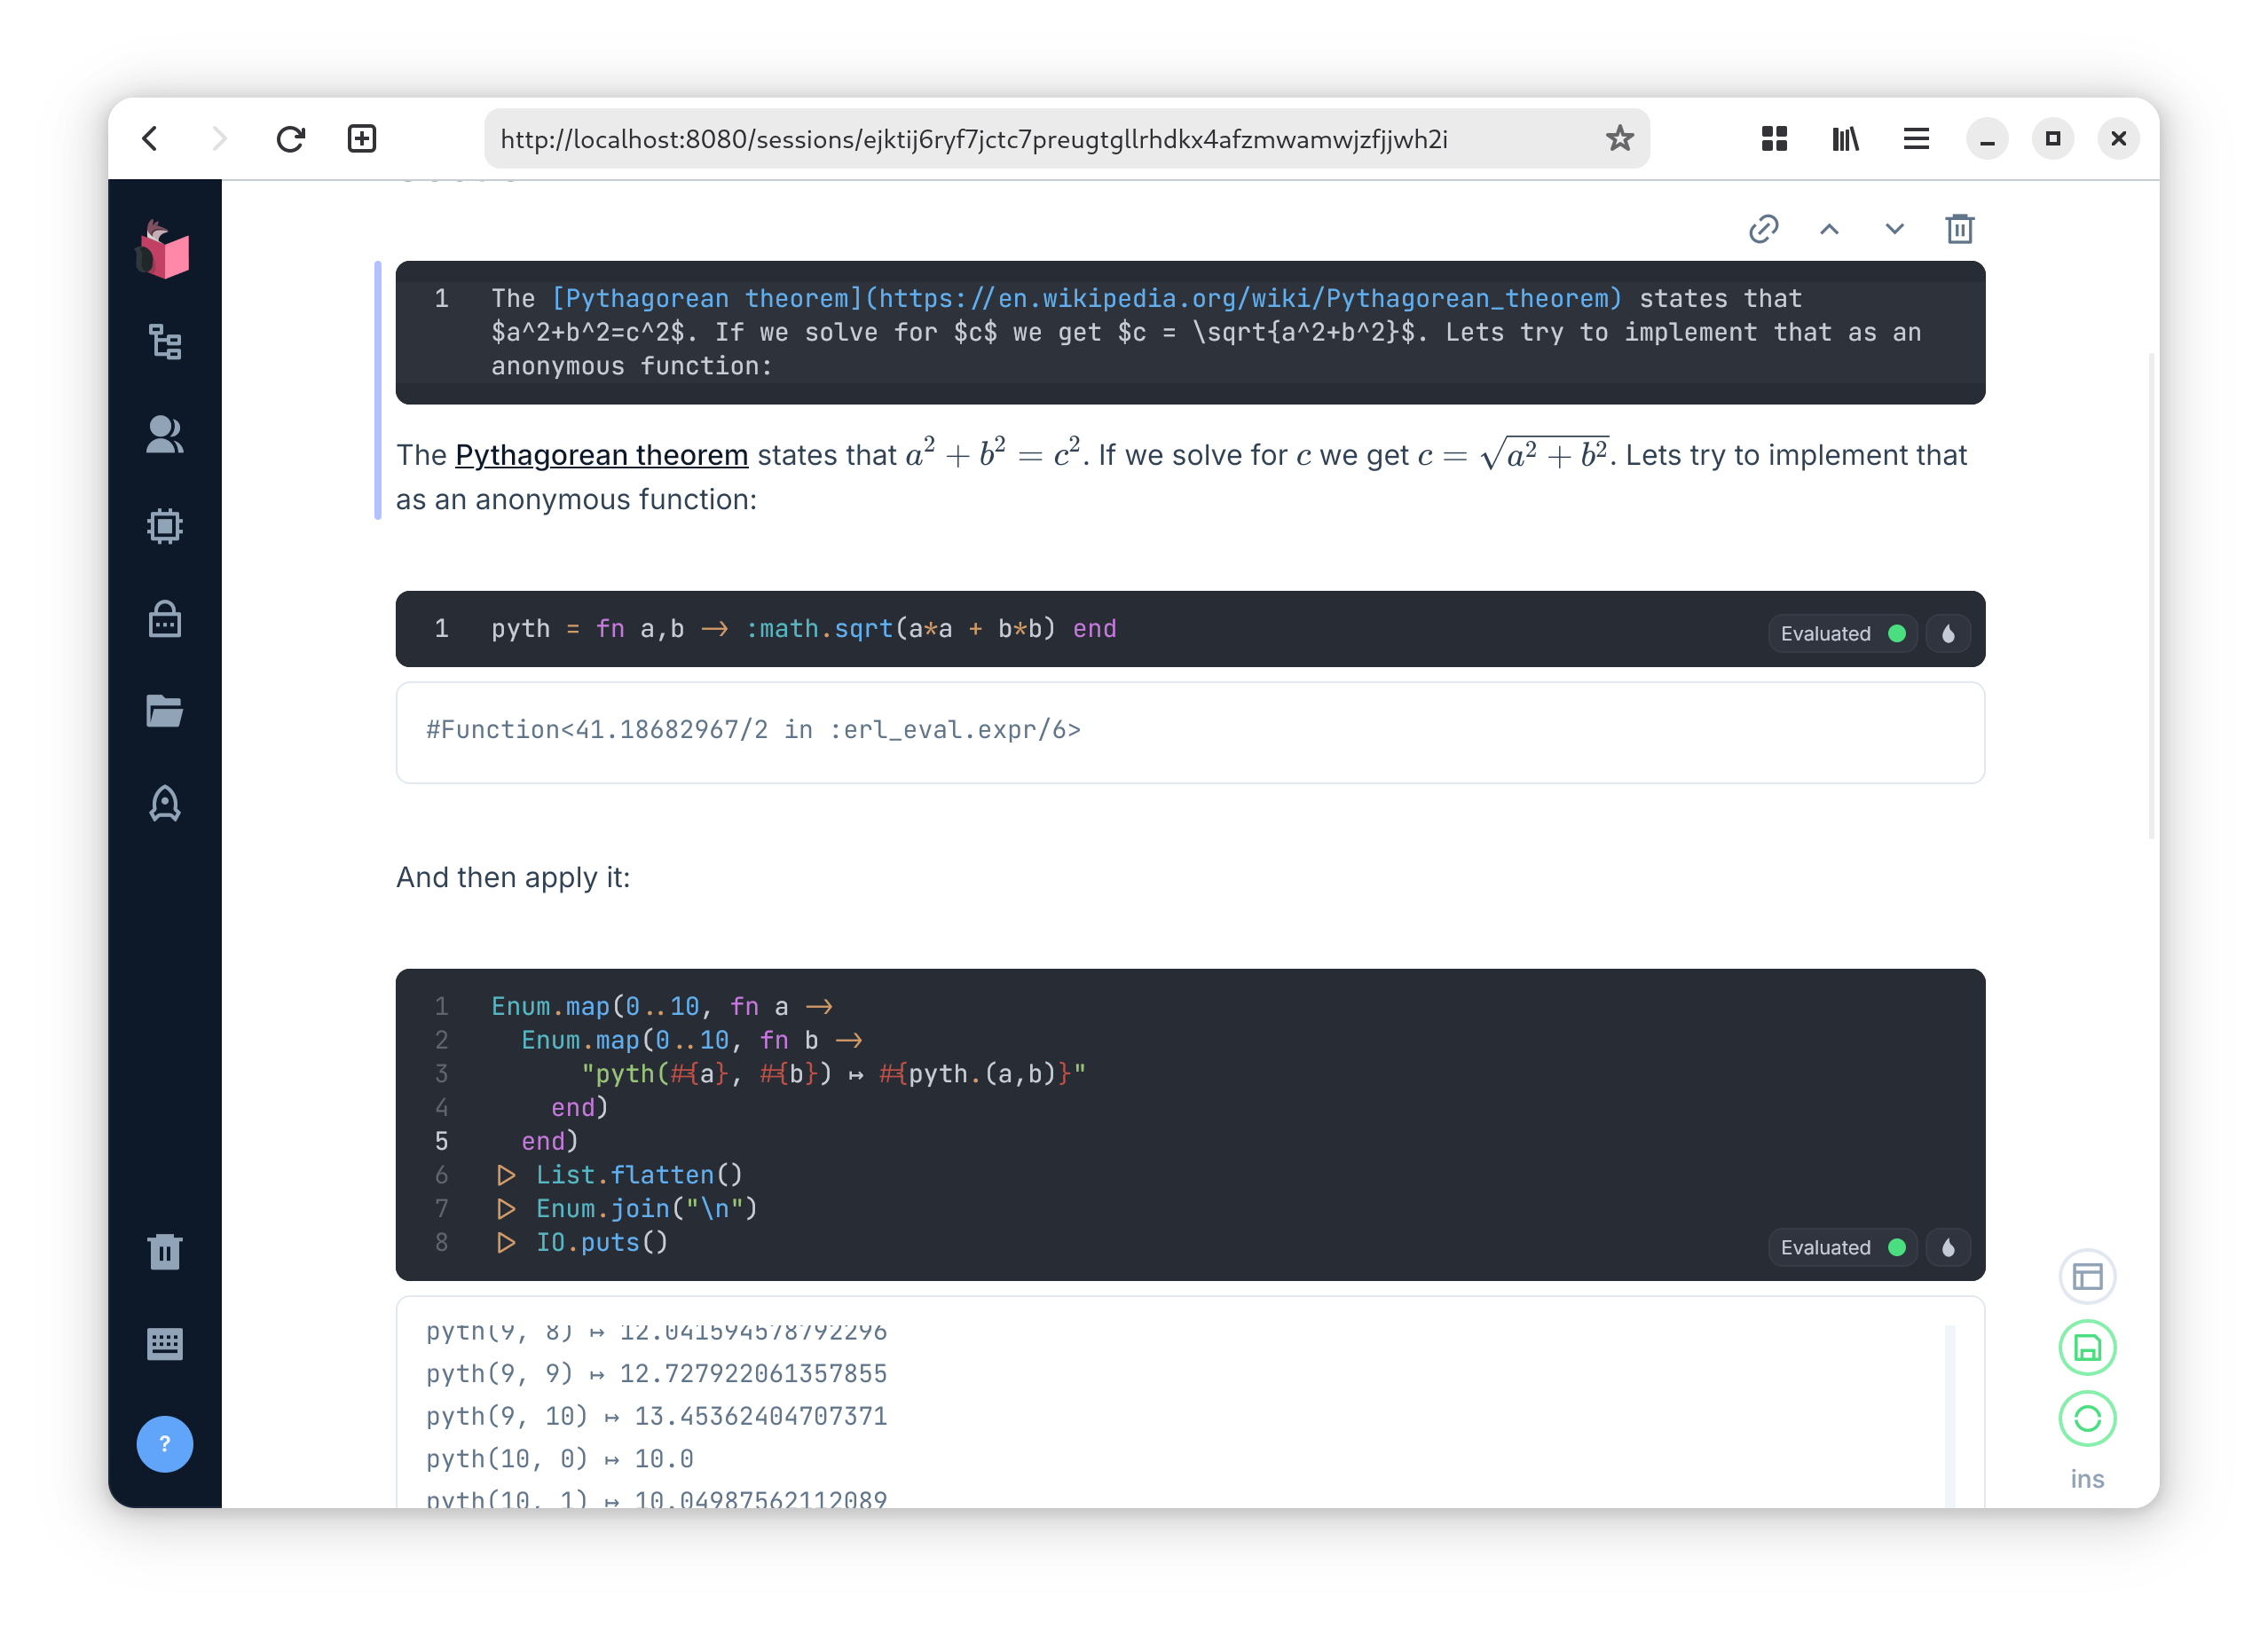
\includegraphics[width=80mm]{./figs/katex-demo.png}
    };
  \end{tikzpicture}
\end{frame}

\subsection{Animation Engines}
\begin{frame}[fragile]
  \frametitle{Animation Engines}
  \vspace{3mm}
  3Blue1Brown:
  \begin{itemize}
    \item Homepage: \textcolor{blue}{\url{https://www.3blue1brown.com}}
    \item Youtube: \textcolor{blue}{\url{https://www.youtube.com/@3blue1brown}}
  \end{itemize}
  
  \pause
  \vspace{5mm}
  Versions:
  \begin{itemize}
    \item Manim:
      \begin{itemize}
        \item Github: \textcolor{blue}{\url{https://github.com/3b1b/manim}}
      \end{itemize}
    \item Manim CE:
      \begin{itemize}
        \item Github: \textcolor{blue}{\url{https://github.com/ManimCommunity/manim}}
      \end{itemize}
  \end{itemize}
\end{frame}

\subsection{Next Level}
\begin{frame}[fragile]
  \frametitle{Next Level}
  \vspace{3mm}
  Proper TeX programming.
  
  \vspace{5mm}
  Constructive methodology for writing \LaTeX\ and dealing with errors.
  
  \vspace{5mm}
  Defining custom \TikZ\ node and edge types.
  
  \vspace{5mm}
  Writing style.
\end{frame}

% background color post
}

%%%%%%%%%%%%%%%%%%%%%%%%%%%%%%%%%%%%%%%%%%%%%%%%%%%%%%%%%%%%%%%
%%%%%%%%%%%%%%%%%%%%%%%%%%%%%%%%%%%%%%%%%%%%%%%%%%%%% Exercises

% background color pre
{
\setbeamercolor{background canvas}{bg=exercises}
\renewcommand{\bgcolor}{exercises}

\section{Exercises}
\begin{frame}
  \vspace{25mm}
  \begin{center}
    \Huge{Part 4:\\Exercises}
  \end{center}
\end{frame}

\subsection{Exercises}
\begin{frame}[fragile]
  \frametitle{Exercises}
  \vspace{1mm}
  \begin{enumerate}
    \descitem{Color Cube:} Use \TikZ\ to draw an RGB color cube that is centered on the page. It should have nodes for red, green, blue, black, cyan, magenta and white, and the appropriate edges.
    \descitem{First Macro:} Lets imagine that you are working on a project where you deal with objects that have a color property. For some reason it is important for you, in a report, to be able to quickly state whether one object is more or less red, green and blue than another. Write a number of macros, that make it easy to write something like this:
      \begin{center}
        $O_1 \overset{\textcolor{red}{\bullet}}{=} O_2$
        \hspace{2cm}
        $O_1 \overset{\textcolor{green!80!black}{\bullet}}{<} O_2$
        \hspace{2cm}
        $O_1 \overset{\textcolor{blue}{\bullet}}{\geq} O_2$
      \end{center}
    \descitem{Automated Test Reporting} Imagine that you have a test suite (e.g., unit tests) and you have to report the outcome as part of the documentation of your work. Pick any test suite that you have lying around. Implement a pipeline that, as part of the build process of a \LaTeX\ document, makes sure to run the tests, parse the results and produce a table with the results that is included in the document.
  \end{enumerate}
\end{frame}

% background color post
}

